\section{Question 3}
\paragraph{(a)} Control law can be computed as
\begin{equation}
	u = -\mathbf{K_x x} + K_r r
\end{equation}
\noindent where $\mathbf{K_x}$ is state gain, $K_r$ is reference gain and $r$ reference signal.

Then, state-space close loop is given by
\begin{align*}
\mathbf{\dot{x}} &= (\mathbf{A}-\mathbf{B K_x})\mathbf{x} + \mathbf{B} K_r u(t), \\
y &= \mathbf{C} \mathbf{x} + \mathbf{D} u(t).
\end{align*}

Time-domain requirements are settling time lower than $4.6$ seconds and $\%PO$ lower than $5\%$. Thus, desired poles are: $\lambda_1 = -5, \lambda_2 = -1, \lambda_3 = -1$. Finally, control gains are
\begin{align*}
\mathbf{K_x} &= 
\begin{bmatrix}
1.8 & 0.8 & 0.4
\end{bmatrix}, \\
\mathbf{K_r} &= 
\begin{bmatrix}
0.3333
\end{bmatrix}.
\end{align*}

Figure \ref{fig:step_response} shows step response of state-space close loop system. The settling time is close to $3.8$ seconds and $\%PO$ is $\%0$.

\begin{figure}[H]
\centering
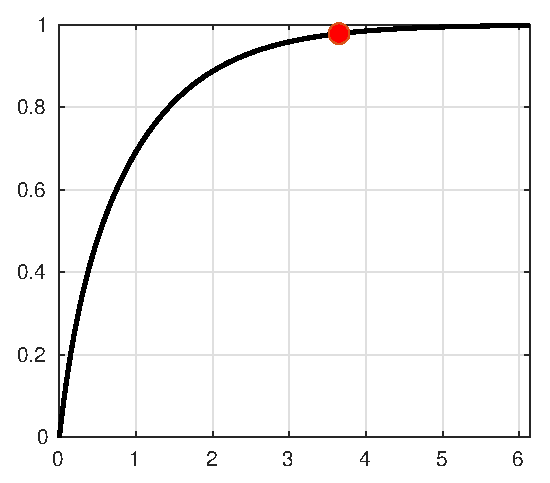
\includegraphics{images/step_response.eps}
\caption{Step response. Settling time is represented with red dot.}
\label{fig:step_response}
\end{figure}











